\documentclass[a4paper,12pt]{article}
\usepackage[backend=biber, citestyle=authoryear, bibencoding=utf8]{biblatex}
\addbibresource{../bibs/external-validity.bib}
\addbibresource{../bibs/econ-causal-history.bib}
\addbibresource{../bibs/causality.bib}
\addbibresource{../bibs/domain-adaptation.bib}
\addbibresource{../bibs/economic-forests.bib}
\addbibresource{../bibs/microcredit.bib}
\addbibresource{../bibs/extra-citations.bib}
\addbibresource{../bibs/quantile-regression.bib}
\addbibresource{../bibs/cash-transfers.bib}
\addbibresource{../bibs/transportability.bib}

\usepackage{amsmath, amsthm, amsfonts, mathtools, csquotes, bm, centernot, bbm}
\usepackage{multirow}
\usepackage[toc,page]{appendix}
\usepackage[hidelinks]{hyperref}

\usepackage{geometry}
\geometry{a4paper, margin=2.5cm}


\theoremstyle{proposition}
\newtheorem{proposition}{Proposition}[section]


% \usepackage[default,light,bold]{sourceserifpro}
\usepackage[T1]{fontenc}

\newtheorem{prop}{Proposition}

\usepackage{pgf, tikz}
\usetikzlibrary{arrows, automata}

\DeclareMathOperator*{\argmax}{argmax}
\DeclareMathOperator*{\argmin}{argmin}
\DeclareMathOperator*{\D}{\mathcal{D}}

\newcommand{\Ex}{\mathbb{E}}
\newcommand{\TTs}{\hat{\tau}(x_i, \Pi, S(d))}
\newcommand{\TTt}{\hat{\tau}(x_i, \Pi, S(d^*))}
\newcommand{\TTsi}{\hat{\tau}(x_i, \Pi, S(d_k))}
\newcommand{\TT}{\tau(x_i, \Pi, d^*)}

\newcommand{\Var}{\mathbb{V}}

\newcommand{\CI}{\mathrel{\perp\mspace{-10mu}\perp}}
\newcommand{\nCI}{\centernot{\CI}}

\title{ Treatment Transfer Trees }

\author{Nandan Rao}


\begin{document}

\maketitle

\begin{abstract}

Internally valid treatment effect studies cannot be used out-of-the-box to predict the effect of the treatment in a new context. Policymakers, however, often need to do just that: predict the effect of a policy in their own context using treatment effect data from other places or times. Few statistical tools exist that explicitly solve this prediction problem.

I extend the Causal Trees framework \parencite{Athey2016} to accept data from multiple domains and modify the objective function to penalize differences across source domains in the dimension splitting process of the tree algorithm. This new algorithm is called Treatment Transfer Trees (TTT). I simulate data to reflect one of the transportability scenarios from \cite{Pearl2014}. In this scenario, the observed data contains a proxy of a latent interacting variable and the functional relationship between them changes from source domain to target domain. On the simulated data, TTT does a significantly better job, compared to a baseline causal tree model, at predicting the effects on the new target domain for which no treatment data exists. The model produces significantly better MSE scores, majority positive as opposed to negative R squared values, and much better confidence interval coverage.

\end{abstract}

\clearpage

\section{Introduction}

Randomized control trials (RCTs), or natural experiments that replicate them, have become the official gold standard of empirical work in economics and many related fields. More and more, policy makers are encouraged to look to RCTs to make ``evidence-based'' policy decisions (\cite{Manski2013, Cartwright2013}).

Many prominent economists have expressed a concern that RCTs and their quasi-experimental colleagues (i.e. natural experiments, instrumental variables, regression discontinuity, etc.) are particularly difficult to generalize to new contexts due to their overarching concern for internal validity, often at the expense of external validity (\cite{Heckman1995, Heckman2008, Deaton2010, Manski2013, Deaton2018}).

Making evidence-based policy decisions is an act of generalizing from previous studies to decisions about the future. Charles Manski \parencite*{Manski2013} voices the concern that experimental studies have tended to ``be silent'' on the question of external validity and that ``from the perspective of policy choice \ldots What matters is the informativeness of a study for policy making, which depends jointly on internal and external validity.''

This silence on external validity means that, despite the huge field of research and techniques for ensuring causal identification (internal validity) via experimental or quasi-experimental methods, very little has been done to either A) create tools to prove that the same results will apply generally in all contexts or B) create tools to predict the results in a specific context, given proven results from one or more experiments.

Abhijit Banjerjee himself \parencite*{Snowberg2016}, a large proponent of RCTs, has recently echoed the current lack of and need for more formal systems for the generalization of experimental studies, stating ``it is our belief that creating a rigorous framework for external validity is an important step in completing an ecosystem for social science field experiments, and a complement to many other aspects of experimentation.''

Predicting the results of a policy in a new location is, tautologically, a prediction problem. Machine learning is a field which has been very successful at formalizing prediction problems. Domain adaptation, a subfield of machine learning, formalizes the problem of moving from one (or more) domains with labelled data to a new domain where only unlaballed data is available (\cite[for a survey, see][]{Pan2010}).

This article extends both the algorithm and the theory of Causal Trees (\cite{Athey2016}) to domain transfer: allowing the algorithm to explicitly incorporate data from multiple domains so as to minimize the predicted error in a new domain. Results from simulated data show that the proposed model outperforms the baseline causal tree model, which could otherwise be a state-of-the-art technique for learning the heterogeneity of treatment effects in one context in order to predict the effect of applying the treatment in a new context.


\section{Prior Art}

Causal Trees (\cite{Athey2016}) extend the basic Classification and Regression Tree (CART) algorithm in two ways: A) they formulate a version of trees to be used with treatment effect data and B) they provide a sample splitting method (``honest estimation'') that provides unbiased estimates and, therefore, accurate confidence intervals through variance prediction of the mean. More than simply extending decision trees, Causal Trees provided the treatment effect community a disciplined way to deal with the multiple testing problem in heterogeneous effect estimation. The insight comes from understanding that the multiple testing problem for coefficient inference is a direct reflection of the overfitting problem for prediction. Thus, the techniques used to prevent predictive overfitting by CART can, in turn, be used to prevent the multiple testing problem in a posterior heterogeneous effect discovery.

% Dahebra et al. and transportability literature!

\cite{Pearl2014} provide a characterization of ``transportability,'' the license to transfer causal effects to a new domain. They show that transportability conditions, given a known causal graph, can be determined by applying some simple do-calculus rules. The conditions return the set of conditional distributions that must be stable across domains in order for the causal effect to transfer.

One scenario is of particular interest is that in which an outcome of interest (which I will simply model as a treatment effect, $\tau$, to avoid any dependence on the do-calculus machinery) has a latent interacting cause $H$. The latent cause has a visible proxy, $V$, and the question is whether or not one can use this visible proxy to predict the treatment effect in a new context

This work extends the Causal Tree framework to provide a prediction tool that can be used effectively in two of the transportability scenarios presented in \cite{Pearl2014}.

\section{Why Trees?}

A regression tree is a well-known technique for building a non-linear model between a potentially high-dimensional set of input covariates and a continous target variable. The Classification and Regression Trees (CART) algorithm is canonically referenced to the original book: \cite{breiman1984classification}, however I would direct a reader without familiarity in the topic to more comprehensive books that put decision trees in the context of other statistical algorithms (i.e. \cite{bishop2006pattern}).

Bishop explains how decision trees use greedy optimization to pick a series of partitions of the input space, in which an individual, very simple, model makes the prediction (for example, the mean response of that partition might be the prediction in a regression tree). The greedy algorithm is the solution provided to overcome the combinatorial problem of the exponential number of ways that a feature space can be divided by recursive binary splits. To overcome local optima, trees are grown to a large depth and later pruned, allowing for initially poor splits to lead to fruitful nodes.

For my purposes, the CART algorithm has several noteworthy properties:

\begin{enumerate}
\item It optimizes over the discrete space of covariates and their interactions with a local, greedy, forward search.
\item It discretizes the continuous input space of covariates.
\end{enumerate}

The optimization implementation implies that at every split of the tree-building process, the CART algorithm is solving the discrete variable selection problem locally based on a defined loss function. Thus, if one can incorporate into the loss function a concept of \textit{domain stability} of the conditional output distribution, the algorithm will pick covariates for which that stability is satisfied locally. This can be contrasted with, for example, a linear model in which the instability of a coefficient across contexts might be driven by only one portion of the input space, whereas the conditional distribution in question might be locally stable in another part. The fact that the algorithm chooses covariates (as opposed to, for example, combining or penalizing them) is attractive in a context where the covariates are thought of as concrete measurements of separable factors that relate somewhat independently to a true underlying causal model\footnote{This feature might also be considered unattractive if one believes that the true causal model operates entirely in a latent space which is jointly dependent on all the input variables.}.

The discretization of the continuous input space of covariates allows for extremely tractable theory regarding treatment effect measurement as well as elegant handling of mixed discrete and continuous covariates.

Finally, regression trees provide a reasonable foundation on which to build a model for domain transfer of treatment effects because of the recent success of Causal Trees (\cite{Athey2016}) and their uptake in both epidimiology and the social sciences. Causal trees allow for non-linear estimation of heterogeneous treatment effects. Heterogeneous treatment effects, being the conditional treatment effect distribution conditional on observed covariates, necessarily form the basis for a transfer model which hopes to transfer to domains in which ovservable covariates differ in distribution.

\section{Problem setup}

The goal is to create an estimator of the true individual treatment effect that performs well in new prediction context, given labelled data in a set of different prediction contexts. The term \textit{domain} will be used instead of ``context'' or ``population'' and I will consider this a problem of domain adaptation in the sense of Ben-David \parencite*{Ben-David2006} and Pan and Yang \parencite*{Pan2010}.

Individual $i$ is characterized by a set of covariates $x_i \in \mathcal{X}$, potential outcomes $y^1_i, y^0_i \in \mathcal{Y}$ from treatment $w_i \in \{0,1\}$, and observed outcome $y_i = w_iy^1_i + (1-w_i)y^0_i$. Individuals belong to separate domains $d \in \mathcal{D}$ with different population distributions $P_d(\tau, X)$.

Denote the average treatment effect (ATE) and the conditional average treatment effect (CATE) for domain $d$ respectively as:
%
\begin{align*}
\tau(d) &\coloneqq \mathbb{E}_{P_d(\tau)}[\tau] \\
\tau(x, d) &\coloneqq \mathbb{E}_{P_d(\tau)}[\tau | X=x]
\end{align*}
%
Assume we have unconfounded samples from from $P_d(X, Y, W)$ for $K$ domains $d \in \mathcal{D_S}$ where unconfounding is defined as $P_d(X, Y^w) = P_d(X, Y | W = w)$. We also have samples from $P_{d^*}(X)$ from domain of interest, $d^* \notin \mathcal{D_S}$.

Our object of interest is:
$$
\tau(X, d^*)
$$
%
In general this is not estimable, $\tau(x, d^*) \stackrel{?}{=} \tau(x, d)$. Our goal is to find a feature-representation function $T: \mathcal{X} \rightarrow \mathbb{R}^M$ for which $\tau(T(x), d^*) \approx \tau(T(x), d)$. To do that, we will search for a $T(\cdot)$ such that $\tau(T(x), d)$ is stable for $d \in \mathcal{D}_S$.

\section{ The data generating process }

To gain some intuition for the problem, it can be helpful to consider a simple scenario which will also form the basis of the simulation studies. Consider a true causal model given by the following directed acyclic graph:

\vspace{5mm}
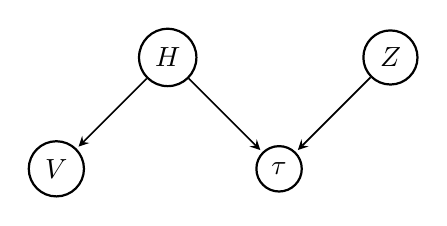
\begin{tikzpicture}[
  > = stealth,
  shorten > = 1pt,
  auto,
  node distance = 2cm,
  semithick
  ]

  \tikzstyle{every state}=[
  draw = black,
  thick,
  fill = white,
  minimum size = 2mm
  ]

  \node[state] (Z) {$Z$};
  \node[state] (t) [below left of=Z] {$\tau$};
  \node[state] (H) [above left of=t] {$H$};
  \node[state] (V) [below left of=H] {$V$};

  \path[->] (Z) edge node {}(t);
  \path[->] (H) edge node {}(t);
  \path[->] (H) edge node {}(V);

\end{tikzpicture}
\vspace{5mm}

\noindent Where $H$ is unobserved, $\tau$ is the treatment effect of interest, and $Z$ and $V$ are both observed variables used in a model $f(Z, V)$ that is used to predict $\tau$.
%
Data is simulated according to the following structural model:
%
\begin{align*}
y_i &= \tau_i W_i + \epsilon_i \\
\tau_i &= f_{\tau}(\alpha, Z_i, \delta,  H_i) \\
Z_i &= \mathcal{N}(Q_{k}, R_{k}) \\
V_i &= C_k H_i + \mathcal{U}(J_{k}, K_{k}) \\
H_i &= \mathcal{N}(A_{k}, B_{k})
\end{align*}

Where $W_i$ is the treatment effect variable and $k \in \{1,...,K\}$ indexes the domain in which the data was generated.

If we consider that $T(\cdot)$ consisted of a simple variable selection problem, we can consider two candidate models that it might want to compare:
%
\begin{align*}
\mathbb{E}_{P_d(\tau)}[\tau | Z, V] &= \int \mathbb{E}_{P_d(\tau)}[\tau | Z, H] \ P(H | V) \ dH \\
\mathbb{E}_{P_d(\tau)}[\tau | Z] &= \int \mathbb{E}_{P_d(\tau)}[\tau | Z, H] \ P(H) \ dH
\end{align*}
%
Due to the assumptions on the causal model, $\mathbb{E}_{P_d(\tau)}[\tau | Z, H]$ will always be stable (it's a generating function). Thus, stability of the considered models is determined by the stability of $P(H)$ and the stability of $P(H | V)$. If $P(H | V)$ is stable, then the full model is naturally prefered. If, however, only $P(H)$ is stable, then the model that omits $V$ (and only considers $Z$) is prefered for prediction in the new domain.

Note that this is completely orthogonal to the requirements for internal validity. An author looking to explain a counterfactual effect in a single domain is perfectly justified using proxy $V$ for true cause $H$ in their model and considering any kind of heterogeneous effects that might be present across different values of $V$. However, any conditional treatment effect that conditions on $V$ will not be necessarily persist to a new domain and thus could create predictions that are arbitrarily poor if shifts in $P(H | V)$ can be arbitrarily large across domains.


\section{ Model }

Denote our estimator of an individuals treatment effect $\hat{\tau}_i$. The oracle squared loss function (where ``oracle'' refers to the fact that $\tau_i$ is unobservable) is given by:
%
$$
\ell(\hat{\tau}, \tau_i) = (\tau_i - \hat{\tau})^2
$$
%
Which is the function this model will try to minimize and is, at this point, equivalent to the objective function of causal trees (\cite{Athey2016}).

Define a discrete partitioning of the feature space, $\Pi \in \mathcal{P}$ where $\mathcal{P}$ denotes the set of all possible partitionings. A discrete partitioning $\Pi$ is defined as a set of $P$ partitions $\{\Pi_1, \dots, \Pi_P\}$ such that:
%
\begin{align*}
\mathcal{X} &= \bigcup\limits_{j=1}^{P} \Pi_j \\
\Pi_a \cap \Pi_b &= \emptyset \ \ \forall \ a,b \in \{1,\dots,P\} \times \{1,\dots,P\}
\end{align*}
%
Denote $\mathcal{S}$ the space of data samples $\{(x_1,y_1,w_1),\dots,(x_N, y_N, w_N)\} \in \mathcal{S}$ Define a random sampling function $S: \mathcal{D} \rightarrow \mathcal{S}$. Notationally denote an expectation of a generic function $g: \mathcal{X}, \mathcal{Y} \rightarrow \mathbb{R}$ taken over the realizations of the sampling function as $\mathbb{E}_S[g(S(d))]$.

Define a ``leaf'' function that finds the correct partition for a given observation:
$$
\lambda(x, \Pi) \coloneqq \{\Pi_j \in \Pi : x \in \Pi_j \}
$$
%
Define a discretized CATE over a set of partitions $\Pi$:
%
$$
\tau(x, \Pi, d) \coloneqq \mathbb{E}_{P_d(\tau)}[\tau | X \in \lambda(x, \Pi))]
$$
%
Define a ``tree'' function that finds the correct partition for a given observation and returns the sample data in that partition, $tree : (\mathcal{X}, \mathcal{P}, \mathcal{S}) \rightarrow \mathcal{S}$:
$$
tree(x_i, \Pi, s) \coloneqq \{(x, y, w) \in s : x \in \lambda(x_i, \Pi) \}
$$
%
Let $\bar{y}^w: \mathcal{S} \rightarrow \mathbb{R}$ return the sample average of all outcomes where $w_i = w$. Define the following estimator $\hat{\tau}: (\mathcal{X}, \mathcal{P}, \mathcal{S}) \rightarrow \mathbb{R}$:
%
$$
\hat{\tau}(\cdot) =  \bar{y}^1(tree(\cdot)) - \bar{y}^0(tree(\cdot))
$$
%
As the sample mean is an unbiased estimate of the expectation, this is an unbiased estimate of $\tau(x,\Pi, d_k)$. In particular, the expectation of the estimate over all possible samples is equal to the true conditional estimate:
$$
\Ex_{S}[\hat{\tau}(x, \Pi, S(d_k))] = \tau(x,\Pi, d_k)
$$
%
Expected oracle loss of a partitioning $\Pi$, given that the conditional treatment estimator is trained on single source domain $d$:
%
$$
\mathbb{E} \ell(\Pi) = \mathbb{E}_{X, S} [ (\tau_i - \hat{\tau}(x_i, \Pi, S(d)))^2  ]
$$
%
Where $\tau_i, x_i \in d^*$ and the expectation is taken over the data to be predicted on the target domain and the samples from the source domain.

\begin{proposition}
The expected oracle loss of a partitioning, $\mathbb{E} \ell(\Pi)$, is estimable given access to $\hat{\tau}(x_i, \Pi, S(d^*))$.
\end{proposition}

\begin{proof} Expanding the square, we can immediately ignore the first term and focus on the second two:
%
\begin{multline*}
\Ex \ell(\Pi) = \Ex_{X} [ \tau_i^2] +  \Ex_{X} [   -2 \Ex_{S}[ \tau_i \TTs] + \Ex_{S}[ \TTs^2 ] ]
\end{multline*}
%
By explicitly writing the expectations over the latter term, we can see that we can re-write it in terms of values we can obtain via sample estimates:
%
\begin{align*}
&= \Ex_{S}[\TTs^2 ]  \\
&=  \Var_{S} [\TTs] +  \Ex_S [\TTs]^2  \\
&\approx  \hat{\Var}_{S} [\TTs] + \TTs ^2
\end{align*}
%
Where we use $\hat{\mathbb{V}}_{S} \coloneqq \frac{s_t^2}{N_t} + \frac{s_c^2}{N_c}$ as a conservative upper bound for the variance \parencite{Imbens2015}. This is an unbiased estimate if the treatment effect is constant and upwardly biased otherwise (as might very well be the case).

We can expand the middle term with the law of iterated expectations and note that, conditional on the value being within a leaf, $\tau_i$ and $\TTs$ become independent:
%
\begin{align*}
-2 \Ex_{X}[ \underbrace{\Ex_{X}[ \tau_i | x_i \in \Pi_j]}_{\approx \hat{\tau}(x_i, \Pi, S(d^*))} \ \underbrace{\Ex_{S}[ \TTs | x_i \in \Pi_j]}_{\approx \hat{\tau}(x_i, \Pi, S(d))}]
\end{align*}
%
Which leads to the loss function, estimable with access to $\hat{\tau}(x_i, \Pi, S(d^*)$:
$$
\sum_j \hat{P}(x_i \in \Pi_j) \bigg( -2 \hat{\tau}(x_i, \Pi, S(d^*)) \TTs  + \hat{\Var}_{S} [\TTs] + \TTs ^2 \bigg)
$$

Where $\hat{P}(x_i \in \Pi_j)$ represents the empirical probability of data $x_i \in d^*$ falling in partition $\Pi_j$.
\end{proof}

This loss is easy to interpret. We'd like to pick leaves in our tree that maximize the cross product between the true average treatment effect in that leaf in our target domain and the expected average treatment effect over our source domains, while not allowing the estimate itself to blow up and at the same time minimizing the variance of the estimator itself.

Unfortunately, we do not have any way to compute the treatment effect on the target domain, where we have no labeled data.

I will make the assumption that the target domain and the source domains are independent realizations of random draws from the same set of possible domains, the same ``domain population,'' $\mathcal{D}$. We will estimate the corresponding part of the loss function with a round-robin approach akin to leave-one-out cross-validation \parencite[See][for an overview of cross-validation]{Hastie2009}:
%
$$
-2 \bigg[ \frac{1}{K} \sum_k^K  \bigg( \hat{\tau}(x_i, \Pi, S(d_k)) \frac{1}{K - 1} \sum_{m \neq k}^K \hat{\tau}(x_i, \Pi, S(d_m)) \bigg) \bigg]
$$
%
This gives us a combined estimated loss function for a given partition $\Pi$ and set of domains $\mathcal{D}$, noting that the loss is equivalent for every prediction $x_i$ in the same leaf, we can come up with a sample estimate of our expected loss $\hat{\ell}(x_i, \Pi, D)$:
%
\begin{multline*}
\sum_{j} \hat{P}(x_i \in \Pi_j) \bigg[ -2   \frac{1}{K} \sum_i^K  \bigg( \hat{\tau}(\Pi_j, S(d_k)) \frac{1}{K - 1} \sum_{m \neq k}^K \hat{\tau}(\Pi_i, S(d_m)) \bigg) \ + \\ \frac{1}{K^2} \sum_k \hat{\Var}_{S} [\TTsi] + \bigg[ \frac{1}{K} \sum_k \TTsi \bigg]^2 \bigg]
\end{multline*}
%
The empirical distribution in the target domain $\hat{P}(x_i \in \Pi_j)$ implies weighting the leaves of our tree by the probability that our target data will fall within the leaf. Note that in the traditional CART algorithm, we would weight our leaves by the number of training data in the leaf. This modification of weights to reflect the $P(X)$ distribution in the target sample is related to importance estimation \parencite{Shimodaira2000} and model variants tested here that use these weights will be referred by the term \textit{importance}.

It should be noted that this expected loss relies heavily on sample averages taken over what are potentially very small number of samples: the number of domains, $K$. In order for the model to be useful in the case where one has very few domains (i.e. 4), I test an alternative formulation:
%
\begin{multline*}
\sum_{j} P(x_i \in \Pi_j) \bigg[ -2   \min_{k \in \{1,\dots,K \}}  \bigg( \hat{\tau}(\Pi_j, S(d_k)) \frac{1}{K - 1} \sum_{m \neq k}^K \hat{\tau}(\Pi_j, S(d_m)) \bigg) \ + \\ \frac{1}{K^2} \sum_k \hat{\Var}_{S} [\TTsi] + \bigg[ \frac{1}{K} \sum_k \TTsi \bigg]^2 \bigg]
\end{multline*}
%
Which I will refer to as the \textit{min} variant. This produces a more conservative estimator when one has few source domains.
%
The prediction by the model is given by the mean of treatment effects within each context in a leaf:
$$
\hat{\tau_i} = \frac{1}{K} \sum_{d_k} \bar{y}^1_{d_k} - \bar{y}^0_{d_k}
$$
And confidence intervals are generated by taking advantage of the variance estimator we have for each individual treatment effect, which are thus easy to accumulate. The intervals are then calculated from a student-t distributioon with degrees of freedom given by the Welch–Satterthwaite equation.

A Python implementation of the model, along with the code to produce the simulation study, is available at: https://github.com/nandanrao/transfer-trees


%

\section{Results}

A linear and three non-linear versions of $f_{\tau}$ from the data generating process is considered:
%
\begin{align*}
f_{\tau}^{linear} &= \alpha V_i  + \delta H_i  \\
f_{\tau}^{nl-hard} &= \alpha V_i \cdot  1 \{ V_i > 0 \} + \delta H_i \cdot  1 \{ H_i > 0 \\
f_{\tau}^{nl-simple} &= \alpha \cdot  1 \{ V_i > 0 \}  +  \delta \cdot 1 \{ H_i > 0 \} \\
f_{\tau}^{nl-stacked} &= \sum_{j=-2}^2 \alpha \cdot  1 \{ V_i > j \}  +  \sum_{j=-2}^2 \delta \cdot 1 \{ H_i > j \}
\end{align*}
%
The following scenarios are considered\footnote{See appendix \ref{appendix:simulation-parameters} for exact simulation parameters.}:
%
\begin{enumerate}
\item $A_{k}, B_{k}$ are constant across all domains. I will refer to this as \textit{Unstable Proxy} or \textit{UP}.
\item $A_{k}, B_{k}, C_{k}, J_{k}, K_{k}$ are constant across all domains. I will refer to this as \textit{Full Stability} or \textit{FS}.
\end{enumerate}
%
I compare the performance of the models with the ``oracle'' treatment effects, impossible to measure in real life but known from the generating process. Rather than compare $R^2$, which would compare the model's performance to the mean in the target domain, I compare the performance to using the (oracle) mean from the source domains:
%
$$
R^2_{tr} \coloneqq 1 - \frac{MSE}{\frac{1}{N} \sum_i (\tau_i - \bar{\tau}_{D_S})^2}
$$
%
This is a reasonable measure to show how well the model solves the transfer problem: if $R^2_{tr}$ is positive, the model has performed better than you could have performed with a perfectly measured (oracle) ATE in your source domain.

In addition to the quantiles for $R^2_{tr}$, I report confidence interval coverage, average tree depth, and a measure of ``feature importance'' for the variable $V$. This is the proxy variable that should be ignored in the UP regime, thus it is informative to see how the TTT models ignore the feature. The results for the simulation study of $K=4$ (4 source domains) and $N=1000$ per domain can be found in table 1.

In the UP regime, the TTT models significantly outperform the CT baseline in all respects with the TTT-M model performing especially well. The most striking performance difference comes in the (90\%) confidence interval coverage of the models in the UP regime. The confidence intervals for the CT baseline hover between 16\%-25\% whereas those for TTT-M hover between 85\%-94\%. In the simple non-linear problem, it returns a positive $R^2_{tr}$ even in the $q=0.1$ quartile and in all the problems it returns strongly positive $R^2_{tr}$ at the $q=0.5$ quartile, whereas the CT baseline hovers around 0 for the more challenging problems. This is all to be expected given the much lower feature importance the TTT models give to proxy variable, $V$, with the TTT-M model giving the lowest importance to that feature of all the models.

Table 2 (appendix) recounts the performance of the model when the number of domains is decreased to 3. In that scenario, the TTT-M model performs even better relative to the others, but the confidence interval coverage suffers being reduced to 77\%-85\%.

In the FS regime, the base treatment transfer tree (TTT) model performs almost identical to the causal tree (CT) baseline, however the TTT-M model underperforms the other two models slightly in this regime. It is overly conservative, growing smaller trees than the other models even though the distributions are not changing between domains.

The treatment transfer tree model with importance estimation performs worse than the other TTT models in all regimes. The exact reason for this is a mystery to me at this point. I hypothesize that it might have something to do with the relative small amount of target data (N), compared with source data (4N).



\begin{table}
\label{tab:results}
\caption{Simulation Results: K=4, N=1000}
\begin{center}
\begin{tabular}{|c|c||c|c|c|c||c|c|c|c|}
\hline
    &  & \multicolumn{4}{|c||}{FS} &  \multicolumn{4}{|c|}{UP} \\
\hline
  &   & linear & hard & simple & stacked & linear & hard & simple & stacked \\
\hline
\hline
\multirow{4}{6em}{$R^2_{t}; q=0.1$}      &    CT &   0.50 &    0.52 &      0.51 &       0.41 &  -1.07 &   -0.77 &     -0.25 &      -0.95  \\
      &   TTT &   0.49 &    0.51 &      0.51 &       0.40 &  -1.02 &   -0.61 &      0.03 &      -0.69  \\
      & TTT-M &   0.43 &    0.46 &      0.48 &       0.24 &  -0.37 &   -0.14 &      0.14 &      -0.28  \\
      & TTT-I &   0.27 &    0.33 &      0.34 &       0.25 &  -1.05 &   -1.12 &     -0.23 &      -1.03  \\
\hline
\hline
\multirow{4}{6em}{$R^2_{t}; q=0.5$}      &    CT &   0.53 &    0.55 &      0.54 &       0.45 &   0.02 &    0.14 &      0.32 &      -0.01  \\
      &   TTT &   0.52 &    0.54 &      0.54 &       0.44 &   0.11 &    0.20 &      0.42 &       0.06  \\
      & TTT-M &   0.48 &    0.50 &      0.52 &       0.34 &   0.14 &    0.22 &      0.44 &       0.11  \\
      & TTT-I &   0.33 &    0.39 &      0.42 &       0.30 &   0.07 &    0.14 &      0.38 &       0.05  \\
\hline
\hline
\multirow{4}{6em}{$R^2_{t}; q=0.9$}      &    CT &   0.55 &    0.58 &      0.57 &       0.48 &   0.49 &    0.55 &      0.64 &       0.45  \\
      &   TTT &   0.55 &    0.57 &      0.57 &       0.48 &   0.42 &    0.53 &      0.63 &       0.32  \\
      & TTT-M &   0.52 &    0.54 &      0.56 &       0.41 &   0.38 &    0.48 &      0.62 &       0.28  \\
      & TTT-I &   0.38 &    0.46 &      0.49 &       0.35 &   0.39 &    0.49 &      0.61 &       0.36  \\
\hline
\hline
\multirow{4}{6em}{$R^2_{t}$; mean}     &    CT &   0.52 &    0.55 &      0.54 &       0.45 &  -0.13 &   -0.01 &      0.25 &      -0.16  \\
     &   TTT &   0.52 &    0.54 &      0.54 &       0.44 &  -0.08 &    0.04 &      0.36 &      -0.08  \\
     & TTT-M &   0.48 &    0.50 &      0.52 &       0.33 &   0.05 &    0.15 &      0.41 &       0.04  \\
     & TTT-I &   0.33 &    0.39 &      0.42 &       0.30 &  -0.14 &   -0.13 &      0.27 &      -0.15  \\
\hline
\hline
\multirow{4}{6em}{V Feat. Imp.} &    CT &   0.57 &    0.47 &      0.64 &       0.60 &   0.56 &    0.52 &      0.59 &       0.60  \\
 &   TTT &   0.58 &    0.46 &      0.63 &       0.59 &   0.41 &    0.34 &      0.28 &       0.49  \\
 & TTT-M &   0.60 &    0.45 &      0.50 &       0.76 &   0.27 &    0.19 &      0.12 &       0.20  \\
 & TTT-I &   0.93 &    0.37 &      0.91 &       0.81 &   0.38 &    0.36 &      0.27 &       0.49  \\
\hline
\hline
\multirow{4}{6em}{CI Coverage}  &    CT &   0.76 &    0.80 &      0.74 &       0.75 &   0.18 &    0.25 &      0.16 &       0.19  \\
  &   TTT &   1.00 &    1.00 &      1.00 &       1.00 &   0.80 &    0.88 &      0.82 &       0.72  \\
  & TTT-M &   1.00 &    1.00 &      1.00 &       1.00 &   0.85 &    0.90 &      0.94 &       0.86  \\
  & TTT-I &   1.00 &    1.00 &      1.00 &       1.00 &   0.69 &    0.80 &      0.82 &       0.75  \\
\hline
\hline
\multirow{4}{6em}{Avg. Depth}   &    CT &   7.57 &    7.52 &      7.04 &       7.37 &   7.79 &    7.60 &      7.41 &       7.61  \\
   &   TTT &   7.51 &    7.40 &      7.07 &       7.46 &   6.61 &    6.66 &      5.64 &       5.53  \\
   & TTT-M &   6.44 &    6.26 &      4.79 &       4.62 &   5.51 &    5.34 &      4.24 &       4.49  \\
   & TTT-I &   8.00 &    8.00 &      8.00 &       8.00 &   6.89 &    6.82 &      7.78 &       7.93  \\
\hline
\end{tabular}
\end{center}
\end{table}


\section{Discussion}

I have shown that it is possible to create a model that learns to transfer treatment effect predictions to a new domain, including in the face of a latent variable and its unstable proxy. This exact data setup is, however, rather constructed and simple. It would be beneficial to test how the model performs as one increases the number of variables and the complexity of the data-generating process.

One particularly interesting regime that was not considered is the one in which the marginal distribution of the latent variable changes, but the

The confidence intervals of the model, while fairly accurate in some of the regimes, are not universally valid even across the relatively limited regimes considered in this paper. Uncertainty prediction is of especial important in the act of predicting across domains where a prior it could be expected that prediction is not possible. More work needs to be done to test the uncertainty quantification and improve its performance across these and more difficult domains.



\printbibliography

\begin{appendices}

\section{Simulation Parameters}
\label{appendix:simulation-parameters}

Parameters for the structural model were simulated as follows:

\begin{align*}
y_i &\coloneqq \tau_i W_i + \epsilon_i \\
\epsilon_i &\sim \mathcal{N}(0, 0.25) \\
\tau_i &\coloneqq f_{\tau}(\alpha, V_i, \delta,  H_i) \\
\alpha &\coloneqq 1 \\
\delta &\coloneqq 0.5 \\
Z_i &\coloneqq \mathcal{N}(Q_{\D}, R_{\D}) \\
Q_{\D} &\sim \mathcal{U}(-2, 4)\\
R_{\D} &\sim \mathcal{IG}(20, 10)\\
V_i &\coloneqq C_{\D} H_i + \mathcal{U}(J_{\D}, K_{\D}) \\
C_{\D} &\sim \mathcal{U}(-2, 2) \\
J_{\D} &\sim \mathcal{U}(-4, 6) \\
K_{\D} &\sim \mathcal{IG}(20, 30) \\
H_i &\sim \mathcal{N}(0, 2)
\end{align*}

\noindent Full code for the simulation available at: https://github.com/nandanrao/transfer-trees

\section{Additional Results}

\begin{table}
\label{tab:results-3}
\caption{Simulation Results: K=3, N=1000}
\begin{center}
\begin{tabular}{|c|c||c|c|c|c||c|c|c|c|}
\hline
    &  & \multicolumn{4}{|c||}{FS} &  \multicolumn{4}{|c|}{UP} \\
\hline
  &   & linear & hard & simple & stacked & linear & hard & simple & stacked \\
\hline
\hline
\multirow{4}{6em}{$R^2_{t}; q=0.1$}      &    CT &   0.48 &    0.50 &      0.50 &       0.40 &  -1.12 &   -0.91 &     -0.29 &      -1.15  \\
      &   TTT &   0.48 &    0.50 &      0.50 &       0.39 &  -1.08 &   -0.70 &     -0.02 &      -0.88  \\
      & TTT-M &   0.45 &    0.47 &      0.49 &       0.29 &  -0.73 &   -0.33 &      0.08 &      -0.68  \\
      & TTT-I &   0.30 &    0.37 &      0.36 &       0.26 &  -1.41 &   -1.05 &     -0.38 &      -1.16  \\
\hline
\hline
\multirow{4}{6em}{$R^2_{t}; q=0.5$}      &    CT &   0.51 &    0.54 &      0.54 &       0.44 &  -0.00 &    0.14 &      0.29 &      -0.07  \\
      &   TTT &   0.51 &    0.53 &      0.53 &       0.43 &   0.15 &    0.24 &      0.40 &       0.04  \\
      & TTT-M &   0.49 &    0.51 &      0.52 &       0.38 &   0.18 &    0.27 &      0.43 &       0.11  \\
      & TTT-I &   0.35 &    0.43 &      0.44 &       0.31 &   0.13 &    0.16 &      0.37 &       0.06  \\
\hline
\hline
\multirow{4}{6em}{$R^2_{t}; q=0.9$}      &    CT &   0.54 &    0.57 &      0.57 &       0.47 &   0.51 &    0.57 &      0.64 &       0.44  \\
      &   TTT &   0.54 &    0.57 &      0.57 &       0.47 &   0.45 &    0.53 &      0.61 &       0.33  \\
      & TTT-M &   0.52 &    0.55 &      0.56 &       0.43 &   0.43 &    0.52 &      0.61 &       0.31  \\
      & TTT-I &   0.41 &    0.48 &      0.49 &       0.36 &   0.48 &    0.51 &      0.58 &       0.39  \\
\hline
\hline
\multirow{4}{6em}{$R^2_{t}$; mean}     &    CT &   0.51 &    0.54 &      0.54 &       0.43 &  -0.18 &   -0.06 &      0.23 &      -0.24  \\
     &   TTT &   0.51 &    0.53 &      0.53 &       0.43 &  -0.11 &    0.04 &      0.34 &      -0.14  \\
     & TTT-M &   0.49 &    0.51 &      0.52 &       0.37 &  -0.01 &    0.11 &      0.37 &      -0.05  \\
     & TTT-I &   0.35 &    0.43 &      0.43 &       0.31 &  -0.19 &   -0.13 &      0.22 &      -0.18  \\
\hline
\hline
\multirow{4}{6em}{V Feat. Imp.}  &    CT &   0.58 &    0.46 &      0.63 &       0.60 &   0.58 &    0.54 &      0.59 &       0.62  \\
 &   TTT &   0.59 &    0.46 &      0.62 &       0.60 &   0.42 &    0.36 &      0.29 &       0.50  \\
 & TTT-M &   0.60 &    0.45 &      0.54 &       0.71 &   0.35 &    0.28 &      0.19 &       0.35  \\
 & TTT-I &   0.94 &    0.36 &      0.91 &       0.79 &   0.39 &    0.35 &      0.28 &       0.46  \\
\hline
\hline
\multirow{4}{6em}{CI Coverage}   &    CT &   0.78 &    0.82 &      0.77 &       0.78 &   0.17 &    0.25 &      0.16 &       0.16  \\
  &   TTT &   1.00 &    1.00 &      1.00 &       1.00 &   0.73 &    0.85 &      0.77 &       0.66  \\
  & TTT-M &   1.00 &    1.00 &      1.00 &       1.00 &   0.77 &    0.87 &      0.85 &       0.75  \\
  & TTT-I &   1.00 &    1.00 &      1.00 &       1.00 &   0.67 &    0.77 &      0.81 &       0.71  \\
\hline
\hline
\multirow{4}{6em}{Avg. Depth}     &    CT &   7.13 &    7.03 &      6.64 &       6.90 &   7.58 &    7.26 &      6.94 &       7.26  \\
    &   TTT &   7.02 &    6.96 &      6.61 &       6.97 &   6.43 &    6.24 &      5.50 &       5.50  \\
    & TTT-M &   6.47 &    6.35 &      5.17 &       5.21 &   5.66 &    5.44 &      4.64 &       4.88  \\
    & TTT-I &   8.00 &    7.99 &      8.00 &       8.00 &   6.97 &    6.86 &      7.60 &       7.77  \\
\hline
\end{tabular}
\end{center}
\end{table}


\end{appendices}


\end{document}